\chapter{INTRODUCTION}
\label{ch:introduction}
\section{Motivation and Background}
Directing a user's attention to objects of interest is a persistent challenge in virtual reality (VR). An immersive environment can surround the user with relevant content, such as targets, instructions, or points of interest, yet only the portion within the current field of view is visible at any moment. Content outside that view must first be brought to the user's attention before it can be inspected or acted on. Prior work has addressed this through subtle gaze guidance that steers attention across an immersive scene~\cite{grogorick2017subtle}, through motion cues that direct attention while preserving immersion~\cite{lange2020hivefive}, and through audio alerts that draw attention to objects of interest~\cite{sabouni2025guidance}. These approaches share a common design problem: how can a system help users locate relevant content without pulling them out of the surrounding environment?

\subsection{Guiding Users Toward Objects of Interest}
Augmented reality (AR) and Virtual reality (VR) technologies have been used in simulation, teleoperation, and entertainment, and provide an immersive setting in which users can identify and interact with objects. Within this setting, the present study explores how the voice used to deliver instructional guidance influences task performance, perceived workload, and enjoyment. It compares self-similar and neutral voices while keeping the content and mechanism of guidance consistent across conditions.

Binetti et al. examine augmented-reality (AR) search assistance motivated by maintenance, repair, instruction, and training, settings in which a person must locate a target in the surrounding scene~\cite{binetti2021outofview}. Zhang et al. examine the concrete example of finding a specified book among other books~\cite{zhang2023seehear}. Such tasks let researchers study how users connect a cue with its intended object without reproducing an entire workplace activity.

Chiossi et al.'s \emph{Searching Across Realities} also studies object search, providing a methodological rationale for using it as a controlled task with behavioral and gaze measures~\cite{chiossi2024searching}. Their study examines how the presentation of physical and virtual content affects search efficiency and attention allocation. For the present comparison, this work motivates specifying the visual environment carefully so that the guiding voice can be varied within a consistent search scene.

When an object begins outside the field of view, assistance must first support attention orientation, directing the user toward a relevant region of the scene~\cite{sabouni2025guidance}. Once that region becomes visible, the user still needs to distinguish the intended object from nearby distractors. This distinction between orientation and local search motivates considering guidance as an unfolding interaction rather than a single cue. Visual techniques offer ways to direct attention~\cite{grogorick2017subtle,lange2020hivefive}; auditory guidance provides another way to communicate where to look as that interaction develops.

\subsection{From Auditory Cues to Spoken Assistance}
Research on auditory guidance supports using sound to help users locate objects, although its benefits depend on the task and cue design. In head-mounted AR, Binetti et al. combined visual arrows with spatialized alarm sounds to guide users toward out-of-view targets~\cite{binetti2021outofview}. Adding sound mitigated response-time costs when visual cues and targets occupied different depth planes, but did not remove the corresponding accuracy cost. The study therefore supports an auditory channel alongside visual guidance, although its cues were alarm sounds rather than speech and it does not show that speech alone is superior to visual cues.

A VR exhibition study compared a rearview mirror, a proximity beep, and a controller vibration against a no-cue control while participants searched for seven target paintings~\cite{sabouni2025guidance}. Audio and haptic alerts reduced how often participants consulted their target list, yet neither shortened completion time relative to the control. These alerts carried minimal information, signaling only that a target was nearby. Spoken guidance can instead specify where to look, which motivates examining speech as a richer channel for orienting attention.

Spoken hints provide a more direct precedent for the present task. Zhang et al.'s AR book-search study used an audio instruction identifying an approximate shelf~\cite{zhang2023seehear}. Hint conditions improved performance relative to the control in the sub-study without post-task feedback, while advantages of combined visual and audio hints depended on task and feedback exposure. Because the verbal cue was delivered at task onset rather than updated in response to gaze, the study motivates spoken search assistance but does not address the more adaptive interaction proposed here.

Gaze-contingent sonification and staged auditory guidance offer complementary precedents for adapting assistance to search progress. Losing et al. varied a tone with gaze-to-target distance, and Kwok et al. combined initial spatial-audio orientation with finer guidance~\cite{losing2014guiding,kwok2022twostep}. Both studies used desktop displays rather than immersive headsets, and their nonverbal cues differ from conversational speech. Their relevance here is the principle of linking the user's current gaze to the information the system supplies next.

Follow My Voice applies this principle through short spoken directions that first orient the participant toward a target region and then refine the search within it. Because the agent knows the target while the participant initially does not know which object to select, speech plays an ongoing instructional role, progressively connecting a direction with the intended object. The participant therefore hears the guiding voice repeatedly during search, which raises a further question: does hearing that guidance in a voice resembling one's own change the experience or effectiveness of receiving help?

\subsection{Self-Similar Voice and the Doppelgänger Connection}
The voice delivering an instruction can influence how users experience an interaction as well as how they engage with a task. Studies of self-similar voices have reported differences in game performance, immersion, and perceptions of a virtual collaborator~\cite{kao2021selfsimilar,guo2024doppelganger}. These findings motivate considering who a guiding voice sounds like alongside what it says. In Follow My Voice, self-similar synthesis creates a cloned voice resembling the participant, allowing the study to examine whether that resemblance changes the experience or effectiveness of receiving spatial instructions.

Kao et al. provide evidence that voice resemblance can affect both behavior and experience~\cite{kao2021selfsimilar}. In an online programming game with 657 analyzed participants, players assigned a self-similar avatar voice completed more puzzles and played for longer than those assigned a dissimilar voice. They also reported greater similarity identification, competence, relatedness, and immersion, although direct differences in the measured intrinsic-motivation subscales were not significant. Performance in that study meant the number of puzzles completed during voluntary play, rather than faster completion of a fixed task. Its findings therefore motivate measuring search performance and experience separately in the present study, without assuming that a self-similar voice necessarily reduces search time.

Guo et al.'s \emph{Collaborating with my Doppelgänger} brings this question into immersive VR~\cite{guo2024doppelganger}. Their 25-participant study crossed self-similar appearance and voice while participants solved a jigsaw puzzle with a virtual character. Self-similar voices increased the character's likability and believability, but also elicited greater eeriness; believability additionally depended on the combination of appearance and voice. This combination of favorable impressions and discomfort is particularly relevant to a guide that speaks repeatedly throughout a task. A familiar-sounding voice may be welcome to one participant and unsettling to another, making both responses important to the evaluation of self-similar assistance.

Evidence from voice listening also connects resemblance with social judgments. Jaggy et al. found that recordings of other speakers whose voices were more similar to a listener's own tended to receive higher likability and trustworthiness ratings~\cite{jaggy2025similarity}. Because this experiment used recorded human voices rather than cloned agents delivering instructions, it supports a possible link between vocal resemblance and agent impressions, rather than demonstrating improved task assistance. Together with the VR findings, it motivates examining how participants perceive the guiding voice alongside how efficiently they find the target.

Voice choice offers a related, but distinct, form of personalization. In \emph{Audio Matters Too}, Kao et al. found that choosing an avatar's voice improved identification and perceived autonomy when participants could also choose its visual appearance; those benefits were not observed without visual choice~\cite{kao2022audiomatters}. This result highlights the importance of the interaction setting and of distinguishing choice from resemblance. Follow My Voice compares a self-similar cloned voice with a neutral voice selected by the participant from the available options. Here, \emph{neutral voice} denotes an existing voice not cloned from the participant; it does not imply emotionally flat speech or an absence of preference. The comparison asks whether self-similar synthesis offers value beyond a voice the user has already chosen, while recognizing that the two voices can differ in naturalness and other acoustic properties as well as resemblance.

The present study extends this literature from an avatar or embodied collaborator to a voice that guides search for an initially unnamed object. Participants use its spatial instructions to determine where to look and what to select, while the agent has no visible body. Perceived voice-similarity ratings assess the intended resemblance; search completion time, workload, motivation, and agent experience address the consequences of receiving guidance in each voice. This design investigates whether self-similar assistance changes the effectiveness or experience of guided search, without presuming an advantage for either condition.

\subsection{A Controlled Setting for Self-Similar Assistance}
Follow My Voice examines this comparison through seated object search in virtual reality. Colored geometric objects are distributed across eight vertical planes around the participant. Some targets initially lie outside the participant's field of view. The application knows which object is the target, while the participant is not given its color or shape at the start. Spoken directions first guide orientation toward the relevant wall and then refine the search within it. The participant aims a right-controller ray and presses the trigger to select the inferred target; gaze itself does not select an object.

Simple geometric shapes on a common arrangement of surrounding planes make starting geometry and trial events easier to specify consistently across the two voice conditions. Object search gives the speech a concrete purpose with observable outcomes, and because the target is initially unnamed, guidance remains consequential until the participant selects it. Applications such as maintenance, training, and everyday retrieval illustrate the broader value of search assistance, although transfer to those settings would require separate evaluation.

The central comparison varies the assigned voice while keeping the assistance mechanism common to both conditions. Gaze contingency and constrained agent decisions use the current search state to select instructions. These shared components provide the setting for examining whether guidance in one's own synthetic voice changes search efficiency or the experience of receiving assistance.

The goal of this thesis is to build on research in attention guidance and voice-based interaction by examining whether self-similar speech has a useful role in spatial assistance. The comparison asks whether hearing instructions in a synthetic version of one's own voice changes the effectiveness or experience of guided search relative to a neutral voice the participant has selected.

Spoken guidance also offers a relevant direction for low-vision assistance because spatial instructions can convey information that would otherwise rely on visible markers. Coughlan et al.'s work with blind users demonstrates the feasibility of verbal corrections for locating points of interest on physical objects~\cite{coughlan2020spatial}. The present method offers a controlled way to study such instruction, but its visual targets and gaze-dependent feedback require separate accessibility testing. An extension for people with low vision would need to consider residual vision, target contrast and size, tracking reliability, and alternatives to gaze-dependent readiness and controller aiming.

\section{Problem Statement}
Previous research explores how visual and auditory guidance can direct attention toward objects of interest, including targets outside the user's current field of view~\cite{grogorick2017subtle,lange2020hivefive,binetti2021outofview,zhang2023seehear}. A related body of work examines how self-similar voices influence the experience of interacting with a virtual agent, including favorable impressions and eeriness~\cite{guo2024doppelganger,kao2021selfsimilar}. Together, these areas motivate examining self-similar spoken assistance in a task where instructions help users discover which object they are seeking.

This study explores the impact of self-similar spoken assistance when guiding search for an initially unnamed object in virtual reality. It evaluates how receiving spatial instructions in a self-similar synthetic voice, compared with a participant-selected neutral voice, affects task performance and the experience of performing the search. The comparison considers active search-completion time, perceived workload, motivation, and agent experience while keeping the task and guidance mechanism consistent across conditions. Because the voices can also differ in naturalness and other acoustic properties, the comparison does not isolate resemblance as their only difference.

Answering this question requires appropriate guidance in both conditions and a record of what each participant actually heard. Gaze contingency, the shared decision policy, and playback logging support this requirement. Independent gaze-quality checks and separate records of looking, pointing, and selecting provide the evidence needed to interpret the interaction~\cite{dunn2024reporting,niehorster2026dataquality}. Chapter~\ref{ch:system}, including Section~\ref{ch:measurement}, describes these controls in support of the central voice comparison.

\section{Research Objectives and Questions}
The primary objective is to evaluate self-similar voice as a form of task assistance, using a neutral voice as the comparison within a shared gaze-contingent system. The primary research question is: will active search-completion time differ between self-similar and neutral voices after accounting for absolute starting angle and repeated observations within participants? The contrast is two-sided because the current design does not justify assuming a performance advantage for self-similarity.

Secondary questions concern perceived workload and activity experience. Will the two voices differ on the six workload dimensions and their complete unweighted mean? Will they differ on interest/enjoyment, effort/importance, pressure/tension, or value/usefulness? Because these outcomes concern different constructs, the analysis will preserve those distinctions rather than pool them into a broad satisfaction score.

Exploratory questions concern agent perception, reliance, and the relationship between task difficulty and voice experience. Participants may describe a voice as more responsive or humanlike, may rely on guidance more often, or may experience a cloned voice as familiar or eerie. Such reports will be treated as judgments about an interaction, not as evidence that the system possesses intelligence, emotions, awareness, or an inner voice.

A supporting validation requirement is to make the assistance process inspectable so that technical faults are not mistaken for effects of self-similar voice. Can recorded state and speech history explain why a cue was eligible, why it played or was suppressed, and how long it waited? Can evaluation distinguish a genuinely unhelpful instruction from an acceptable alternative wording? These questions concern system validity and readiness; they support the empirical study but do not replace it.


\subsection{Research-Question Traceability}
Each question carries a stable identifier so that the completed results and conclusion can answer the questions as they are posed here. RQ1 is the primary empirical contrast, RQ2 concerns secondary experience measures, and RQ3 is exploratory; EQ1 is an engineering question rather than a fourth participant research question. Table~\ref{tab:rq-map} connects each question to its evidence and analysis. The identifiers organize the existing plan without adding an experimental factor or a directional hypothesis.

\begin{table}[htbp]\centering
\caption[Research questions and evidence requirements]{Research-question traceability for the proposed study. No empirical answer is available in this first pass.}
\label{tab:rq-map}
\small\tagpdfsetup{table/header-rows={1}}
\begin{tabularx}{\linewidth}{@{}p{0.12\linewidth}p{0.39\linewidth}X@{}}\toprule
Question & Intended contrast & Evidence and reporting destination \\\midrule
RQ1 & Does self-similar voice change active completion time relative to a neutral voice? & Trial timing and starting geometry; analysis in Section~\ref{ch:analysis}, results in Chapter~\ref{ch:evaluation}. \\
RQ2 & Do self-similar and neutral voices differ in workload or motivation? & Paired block-referenced workload and separate IMI subscales; final retrospective administration. \\
RQ3 & How do voices differ in agent perception, voice experience, reliance, and search behavior? & Custom ratings, agent constructs, debrief, and valid search measures; exploratory voice-by-angle comparison. \\
EQ1 & Can the recorded sequence explain eligibility, delivery, and unhelpful guidance? & State, request, and actual playback records; sequence tests and evaluation rubric in Appendix~\ref{app:scenarios}. \\\bottomrule
\end{tabularx}
\end{table}

The voice-similarity manipulation check will be reported before the outcome contrasts because it informs the interpretation of every question; it will not be used to exclude individual participants. RQ3 also covers appealing, eerie, and familiar impressions of the voice and the exploratory question of whether the voice contrast varies with starting angle.

\section{Scope of the Comparison}
The independent variable is voice condition: neutral voice versus self-similar synthetic voice. Both conditions use gaze contingency, the same semantic phrase library, the same local geometry rules, and the same controller-selection mechanics. Because these are shared system properties, the study will not isolate the contribution of gaze contingency, short-term memory, the cloud decision agent, or synthetic speech in general.

The task is deliberately narrower than unrestricted navigation. Participants remain seated and rotate their head and chair to search surrounding planes. Guidance such as ``turn left'' concerns orientation within this setup; it does not ask them to walk toward a target. Objects appear in a virtual room, and the target is initially unnamed. Conclusions will therefore be bounded to guided search under these conditions.

Under the current protocol, the single practice trial uses the first assigned voice. This introduces an exposure asymmetry, because whichever voice appears first is also heard during practice. Counterbalancing distributes that asymmetry across voices but does not remove learning or carryover, so the analysis will retain period and assigned order, and the report will describe the practice assignment explicitly.

Figure~\ref{fig:comparison-framework} separates the voice manipulation from the shared task; it specifies the comparison without predicting its direction.

\begin{figure}[htbp]
\centering
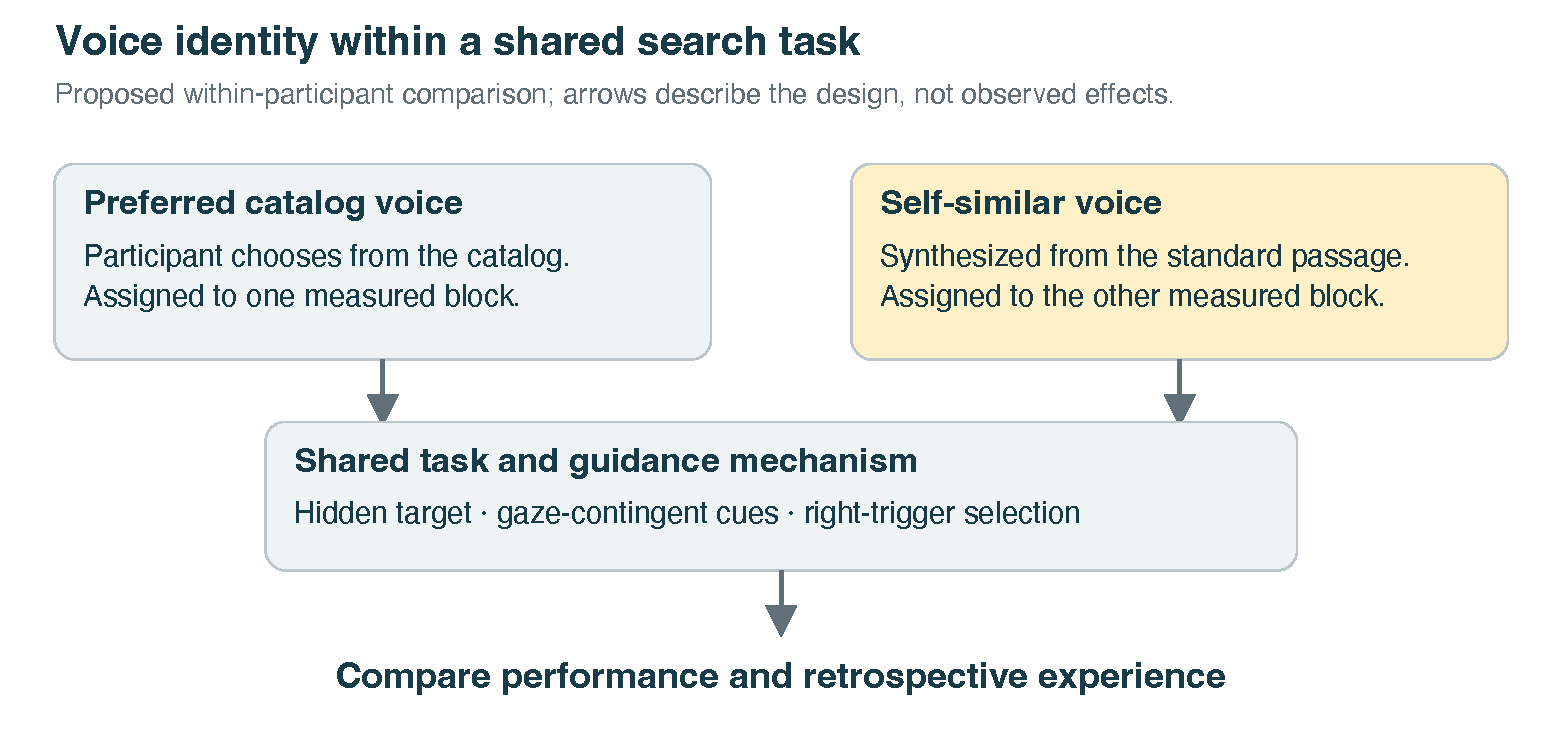
\includegraphics[width=\linewidth,alt={Two voice conditions feed a shared hidden-target search task and a paired outcome comparison.}]{figures/comparison-framework.pdf}
\caption[Voice comparison within the shared search task]{Proposed comparison of neutral and self-similar voices within a shared task and guidance mechanism. The schematic identifies the intended manipulation and outcome families; it does not depict observed effects.}
\label{fig:comparison-framework}
\end{figure}


\section{Intended Contributions}
The thesis develops an empirical comparison of self-similar voice with a preferred alternative in virtual-reality task assistance. Its conceptual contribution is to distinguish resemblance from preference and to examine performance alongside the favorable or uncomfortable experience of hearing one's own synthetic voice. The study will not assume that greater perceived similarity implies faster search, lower workload, or a more welcome agent.

The methodological contribution is a within-participant design that makes this comparison operational: two counterbalanced voice blocks, a shared hidden-target task, explicit trigger selection, identical nominal starting-angle quotas across blocks, retrospective voice-referenced questionnaires, and a planned repeated-measures analysis. Manipulation checks and acoustic-quality reporting will help establish what the voice conditions actually delivered before their outcomes are interpreted.

The implemented guidance and recording platform supports that empirical contribution. Local spatial eligibility, constrained agent decisions, prepared speech, and synchronized review make it possible to inspect what each participant heard and whether delivery problems affected the comparison. The platform serves as the apparatus for studying self-similar voice; the thesis does not present a provider benchmark or a new gaze-guidance algorithm as its primary contribution.

The empirical contribution remains pending: this draft reports no recruited sample, condition means, significance tests, or participant quotations. The completed thesis will replace the pending results sections with the actual voice-condition outcomes of the frozen study and revise its abstract and conclusion accordingly.

\section{Organization of the Thesis}
Chapter~\ref{ch:literature} connects XR applications, attention guidance, gaze interaction, and self-similar voice research. Chapter~\ref{ch:system} presents the methodology, including application design, the experiment and procedure, data collection, scoring, and the planned analysis. Chapter~\ref{ch:evaluation} organizes results into performance, experience, and supporting engineering evidence, with participant outcomes pending. Chapter~\ref{ch:discussion} considers interpretation, limitations, and future work, and the conclusion returns to the research questions. The appendices preserve questionnaire instruments, data definitions and scoring rules, and guidance sequence tests.
